% begin module tangents-ex1
\begin{frame}
\begin{example}[Example 1, p. 113]
Find an equation for the tangent line to the parabola $y = x^2$ at the point $P = (1,1)$.

\begin{columns}[c]
\column{.4\textwidth}
\ \uncover<9->{%
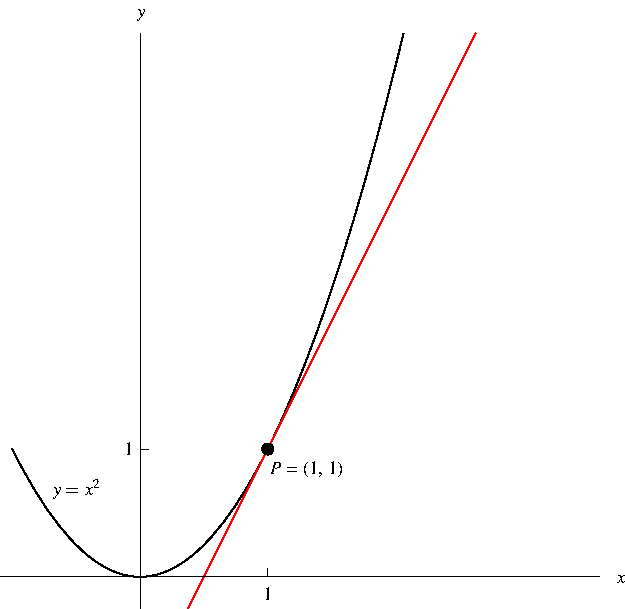
\includegraphics[height=4.5cm]{derivatives/pictures/02-01-secanta.pdf}%
}%
\column{.6\textwidth}
\uncover<2->{%
Here $a = 1$ and $f(x) = x^2$.
}%
\begin{eqnarray*}
\uncover<3->{m} & \uncover<3->{ = } & \uncover<3->{\lim_{x\rightarrow 1} \frac{f(x)-f(1)}{x-1}}\\
& \uncover<4->{ = } & %
\uncover<4->{\lim_{x\rightarrow 1}\frac{x^2 - 1}{x-1}}\\
& \uncover<5->{ = } & %
\uncover<5->{\lim_{x\rightarrow 1}\frac{(x - 1)(x+1)}{x-1}}\\
& \uncover<6->{ = } & %
\uncover<6->{\lim_{x\rightarrow 1}(x+1)}\uncover<7->{ = 1 + 1 = 2}
\end{eqnarray*}
\uncover<8->{
Point-slope form: $y - 1 = 2(x - 1)$, or $y = 2x - 1$.
}
\end{columns}
\end{example}
\end{frame}
% end module tangents-ex1
